\documentclass{article}

\usepackage[utf8]{inputenc}
\usepackage[brazilian]{babel}
\usepackage{graphicx}
\usepackage{float}
\usepackage[pdftex]{hyperref}
\usepackage{epstopdf}
\usepackage{etoolbox}
\usepackage{amsmath}
\usepackage{amsfonts}
\usepackage{amssymb}
\usepackage{caption}
\usepackage{subcaption}
\usepackage{setspace}
\usepackage{tikz}

\patchcmd{\thebibliography}{\section*}{\section}{}{}
\newcommand{\R}{\ensuremath{\mathbb{R}}}
\newcommand{\Prob}{\ensuremath{\mathbb{P}}}
\newcommand{\K}{\ensuremath{\mathbb{K}}}
\newcommand{\U}{\ensuremath{\mathbb{U}}}
\newcommand{\N}{\ensuremath{\mathbb{N}}}
\newcommand{\Lg}{\ensuremath{\mathbb{L}}}
\newcommand{\T}{\ensuremath{\rm Tr}}
\newcommand{\sg}{{\sigma(x_k)}}

\newcommand{\G}{\ensuremath{\mathcal{G}}}
\newcommand{\F}{\ensuremath{\mathcal{F}}}
\newcommand{\C}{\ensuremath{\mathcal{C}}}
\newcommand{\E}{\ensuremath{\mathcal{E}}}
\newcommand{\Hn}{\ensuremath{\mathcal{H}}}
%\newcommand{\Hoo}{\ensuremath{\mathcal{H}_\infty}}
\newcommand{\Hop}{\ensuremath{\mathcal{H}_{op}}}
% --------------------------------------------------
\newtheorem{theo}{Teorema}
\newtheorem{exa}{Exemplo}
\newtheorem{lemm}{Lema}
\newtheorem{coro}{Corolário}
\newtheorem{defn}{Definição}[section]

%opening


\begin{document}
\input{capa.tex}

\onehalfspacing
\section{Objetivos} 
O objetivo desse experimento é realizar a identificação de parâmetros de um sistema torcional composto por dois discos interligados por uma haste flexível acionados por um motor de corrente contínua,conforme modelo proposto no roteiro\cite{bb:roteiro}. As posições angulares dos discos são medidas por dois encoders, e o motor é acionado pelo modulador de largura de pulso (PWM).
	
\section{Modelo matemático}
O modelo problema é mostrado no esquema da figura \ref{fig:esqmotor} e está descrito pelas equações \ref{eq:eletrica}, \ref{eq:disco1} e \ref{eq:disco2}. Para este experimento, iremos considerar que o indutor é carregado instantaneamente, ou seja, que $L=0$. Também adotaremos as variáveis de estado do sistema como $x_1=\theta_1-\theta_2$, $x_2=\dot{\theta_1}$ e $x_3=\dot{\theta_2}$.

\begin{figure}[H]
	\centering
	\includegraphics[width=0.8\linewidth]{esqmotor}
	\caption{Esquema do motor (elétrica e mecânica)}
	\label{fig:esqmotor}
\end{figure}

\begin{equation}
\label{eq:eletrica}
L\dot{i}+Ri+K\dot{\theta_1}=V
\end{equation}
\begin{equation}
\label{eq:disco1}
(J_1)\ddot{\theta_1}+b_1\dot{\theta_1}+\kappa(\theta_1-\theta_2)=Ki
\end{equation}
\begin{equation}
\label{eq:disco2}
(J_2)\ddot{\theta_2}+b_2\dot{\theta_2}+\kappa(\theta_2-\theta_1)=0
\end{equation}

\begin{equation}
\label{eq:ss}
\left[ \begin{array}{c}
\dot{x_1} \\
\dot{x_2} \\
\dot{x_3} \end{array} \right]
=
\left[ \begin{array}{ccc}
0 & 1 & -1 \\
-\frac{\kappa}{J_1} & -\frac{(b_1+K^2/R)}{J_1} & 0 \\
\frac{\kappa}{J_2} & 0 & -\frac{b_2}{J_2} \end{array} \right]
\left[ \begin{array}{c}
x_1 \\
x_2 \\
x_3  \end{array} \right]
+
\left[ \begin{array}{c}
0 				\\
\frac{K}{RJ_1} 	\\
0				\end{array} \right]
V
\end{equation}

\section{Ensaio com motor travado}
Conforme o roteiro\cite{bb:roteiro}, ao ligar o motor com o disco ligado a ele travado não geramos força contra-eletromotriz, e com isso conseguimos medir a corrente de armadura $i$ com a adição de um resistor $R_s$. Isso nos possibilita o cálculo do parâmetro $R [\Omega]$ (soma da resistência do motor e $R_s$) pela equação \ref{eq:rotparado}. Adotaremos a indutância $L=0$.

\begin{equation}
\label{eq:rotparado}
i(t) = \frac{V}{R}
\end{equation}

Travando o disco 1 para impossibilitar o motor de girar seu rotor, fizemos o acionamento do módulo de potência, aguardamos a estabilização do sinal de corrente, e desligamento do sistema, obtendo a curva de corrente mostrada na figura \ref{fig:ensaiop}. Destacamos o valor da corrente quando estável para facilitar a análise.

\begin{figure}[H]
	\centering
	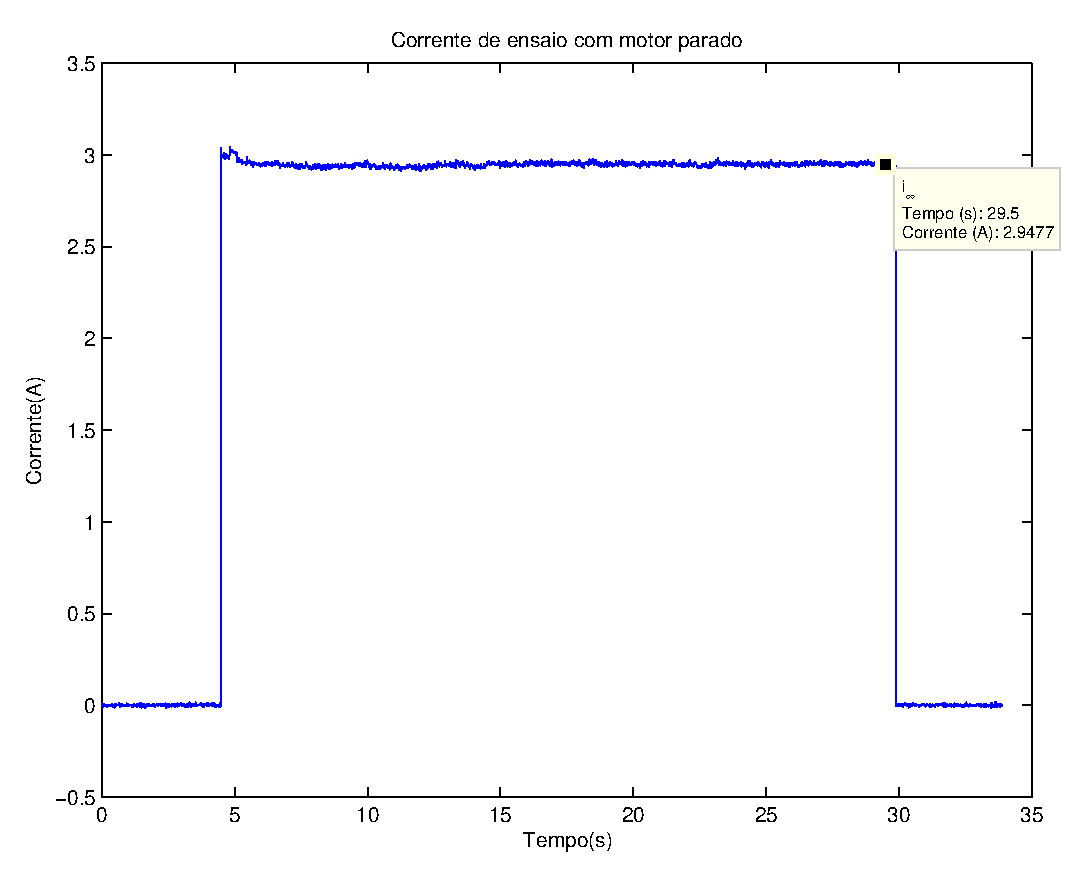
\includegraphics[width=0.8\linewidth]{../ensaiop}
	\caption{Corrente de ensaio com motor travado}
	\label{fig:ensaiop}
\end{figure}

Para o cálculo do parâmetro $R$, utilizamos a tensão da fonte $V=12 V$ e a partir do momento em que a corrente se estabiliza em $i_\infty=2.9477A$, calculamos seu valor conforme \ref{eq:r}.

\begin{equation}
\label{eq:r}
R = \frac{V}{i_\infty}=4.0709\Omega
\end{equation}

\section{Ensaio com motor em movimento}
Agora sem travar os discos, acionamos o módulo de potência e aguardamos a estabilização do sinal de corrente e velocidade, e desligamos o sistema, obtendo a curva de corrente mostrada na figura \ref{fig:ensaiori} e a curva de velocidade angular do disco 1 mostrada na figura \ref{fig:ensaiorv}.

\begin{figure}[H]
	\centering
	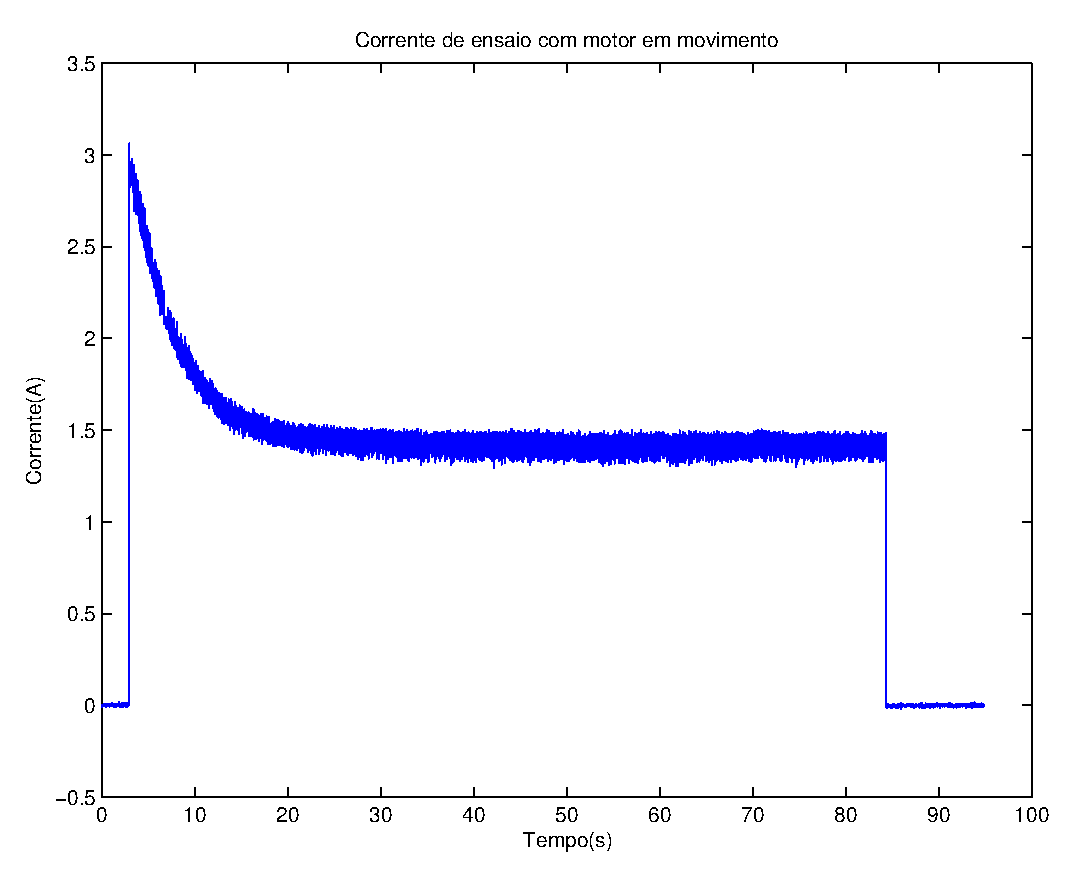
\includegraphics[width=0.8\linewidth]{../ensaiori}
	\caption{Corrente durante ensaio com motor em movimento}
	\label{fig:ensaiori}
\end{figure}

\begin{figure}[H]
	\centering
	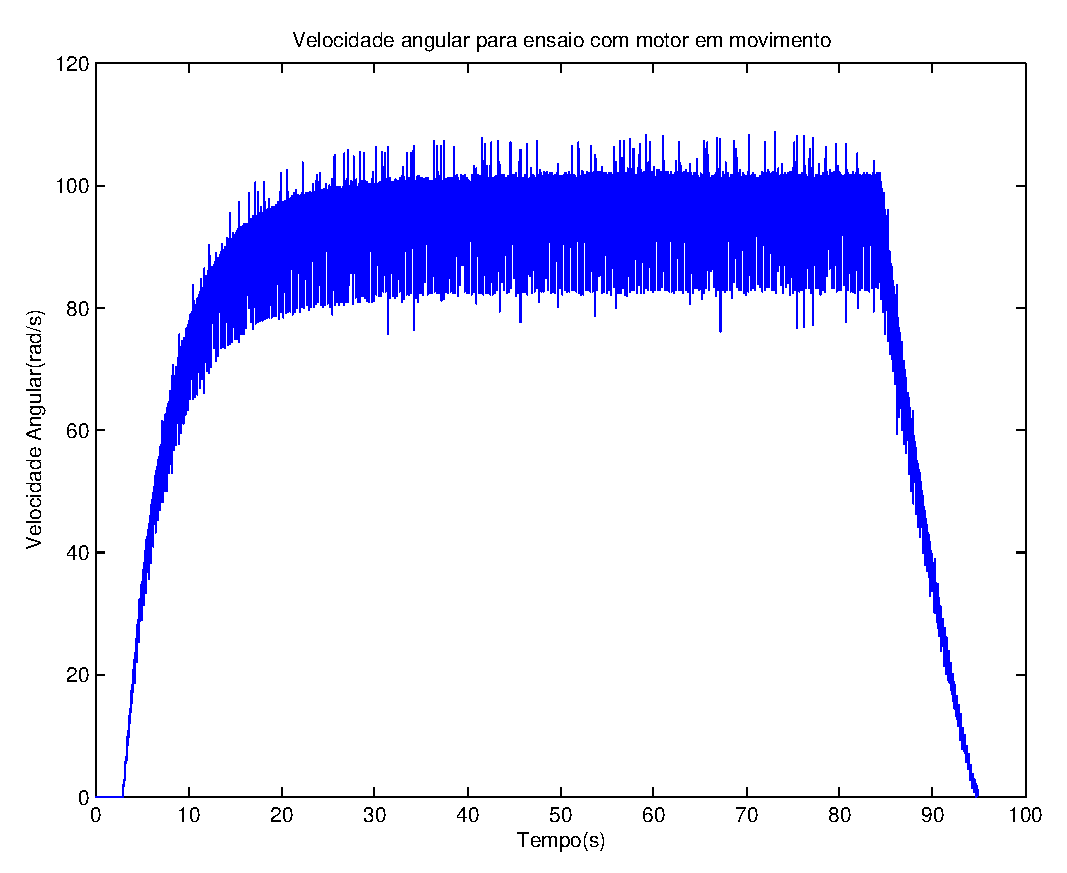
\includegraphics[width=0.8\linewidth]{../ensaiorv}
	\caption{Velocidade angular do disco 1 durante ensaio com motor em movimento}
	\label{fig:ensaiorv}
\end{figure}

Filtramos os sinais e destacamos as medidas em regime permanente para facilitar a análise, como pode ser visto nas figuras \ref{fig:ensaioriF} e \ref{fig:ensaiorvF}.
\begin{figure}[H]
	\centering
	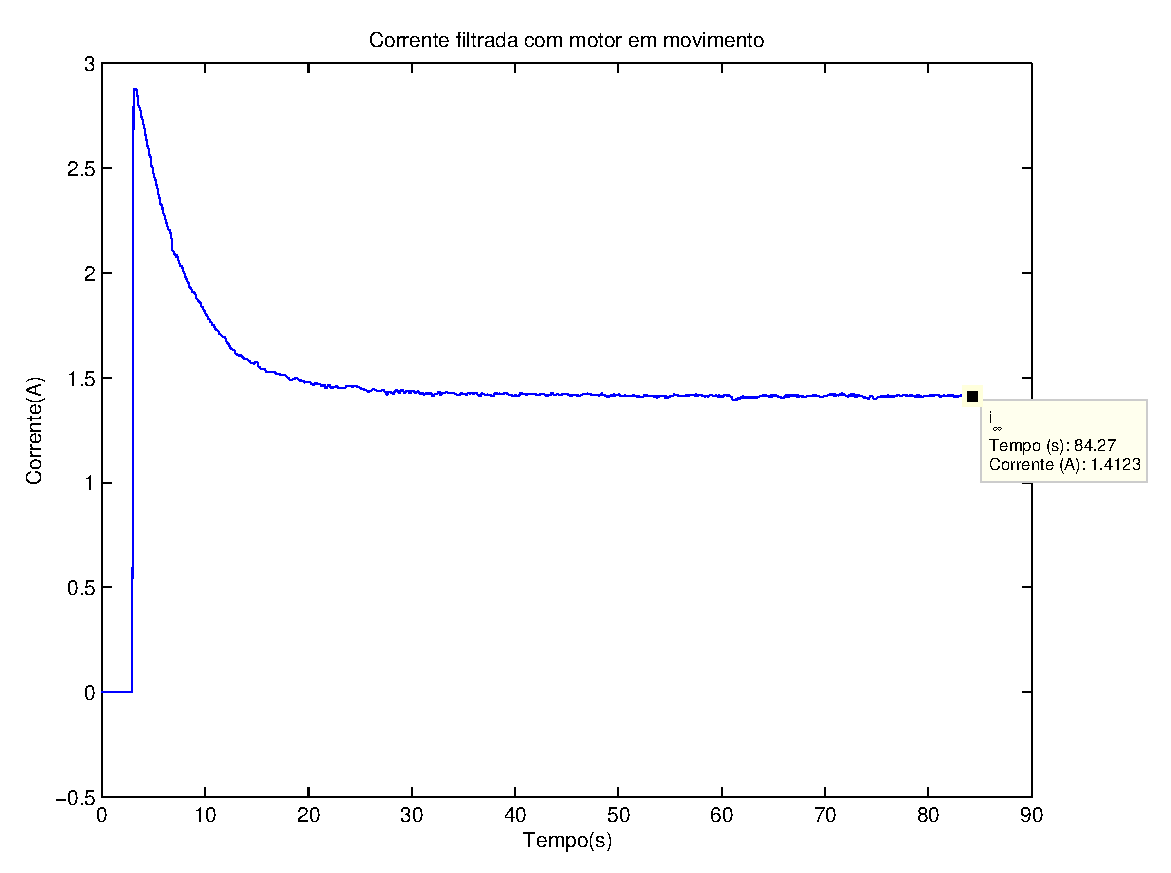
\includegraphics[width=0.8\linewidth]{../ensaioriF}
	\caption{Corrente filtrada para ensaio com motor em movimento}
	\label{fig:ensaioriF}
\end{figure}

\begin{figure}[H]
	\centering
	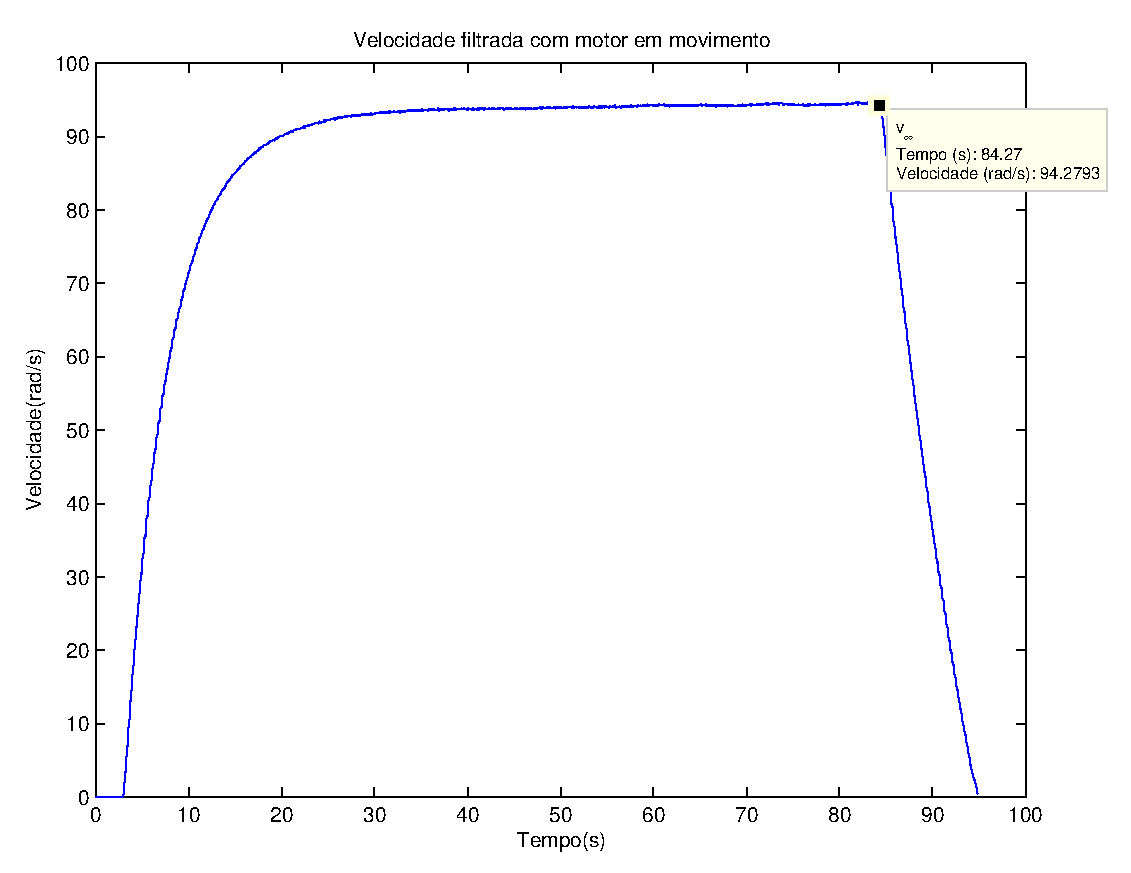
\includegraphics[width=0.8\linewidth]{../ensaiorvF}
	\caption{Velocidade angular do disco 1 filtrada para ensaio com motor em movimento}
	\label{fig:ensaiorvF}
\end{figure}

Esperando a velocidade do motor se estabilizar, chegamos em $\nu_{\infty}=94.2793rad/s$. Considerando que a esse ponto o indutor se comporte como curto circuito, encontramos a constante de torque do motor conforme a equação \ref{eq:k}

\begin{equation}
\label{eq:k}
K=\frac{V-Ri_{\infty}}{\nu_{\infty}}=0.0663 V\cdot s
\end{equation}

Encontramos também a soma dos coeficientes de atrito viscoso $b_1$ e $b_2$, utilizamos as equações \ref{eq:eletrica}, \ref{eq:disco1} e \ref{eq:disco2}, fazendo $\ddot{\theta}=0$, chegando à equação \ref{eq:b1b2}.

\begin{equation}
\label{eq:b1b2}
b_1+b_2=\frac{K}{R}\left(\frac{V-K\nu}{\nu}\right)=9.9316\cdot10^{-4}
\end{equation}

\section{Ensaio com motor desligado}
Com o motor desligado, travamos o disco do lado sem motor, tiramos o disco do lado com motor da posição de equilíbrio e soltamos, obtendo seu deslocamento angular conforme mostrado na figura \ref{fig:disco2travado}. Fazendo o processo equivalente para o outro disco obtivemos o resultado mostrado na figura \ref{fig:disco1travado}.

\begin{figure}[H]
	\centering
	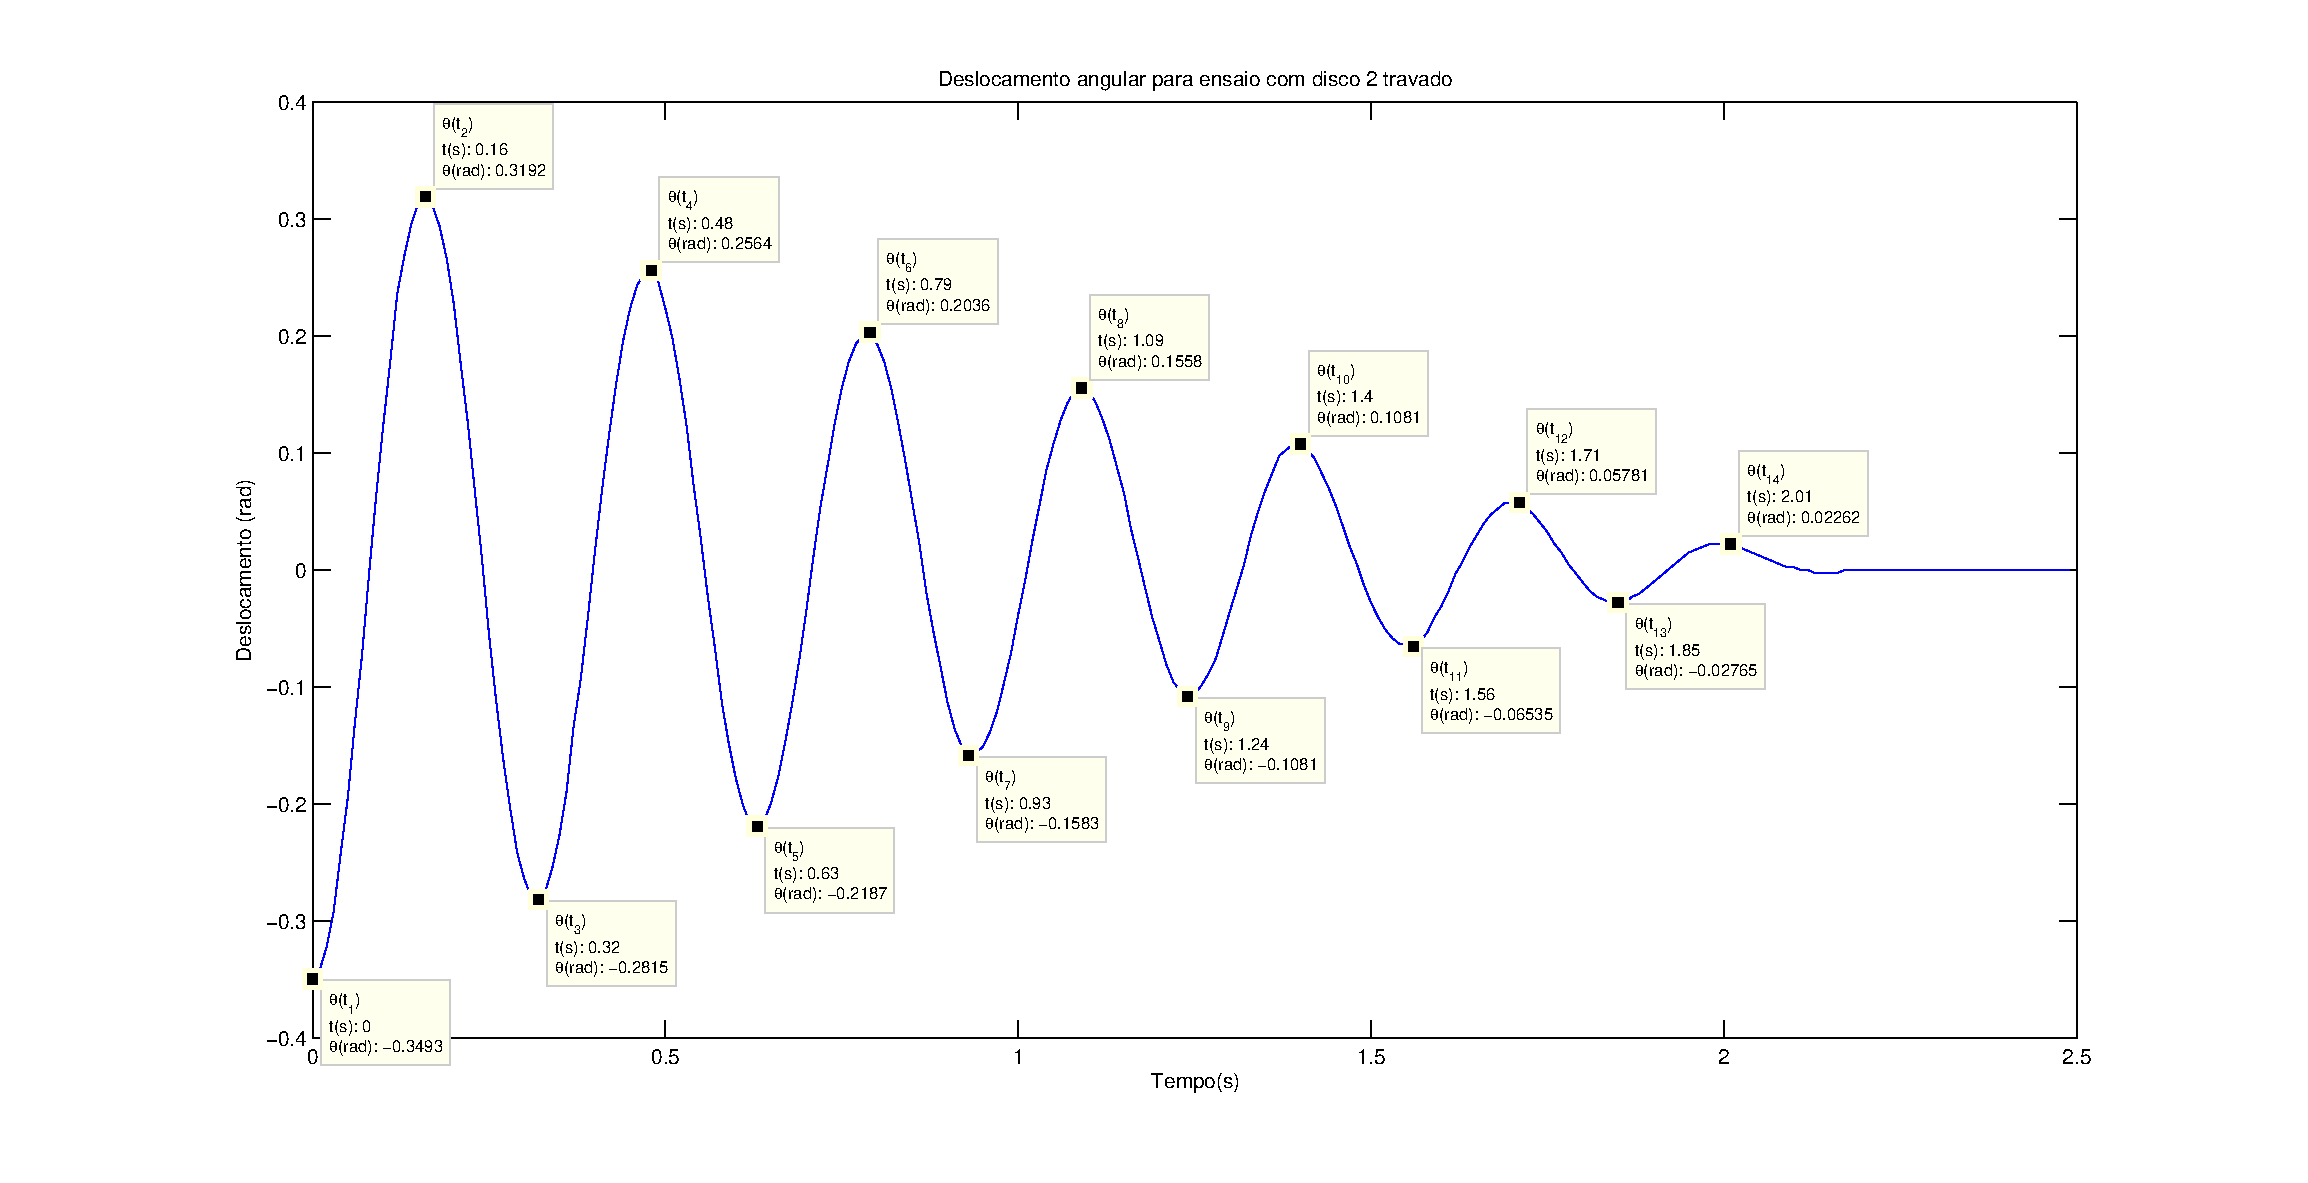
\includegraphics[width=0.8\linewidth]{../disco2travado}
	\caption{Pontos de relevância para deslocamento angular em oscilação do disco 1 (lado com motor)}
	\label{fig:disco2travado}
\end{figure}
\begin{figure}[H]
	\centering
	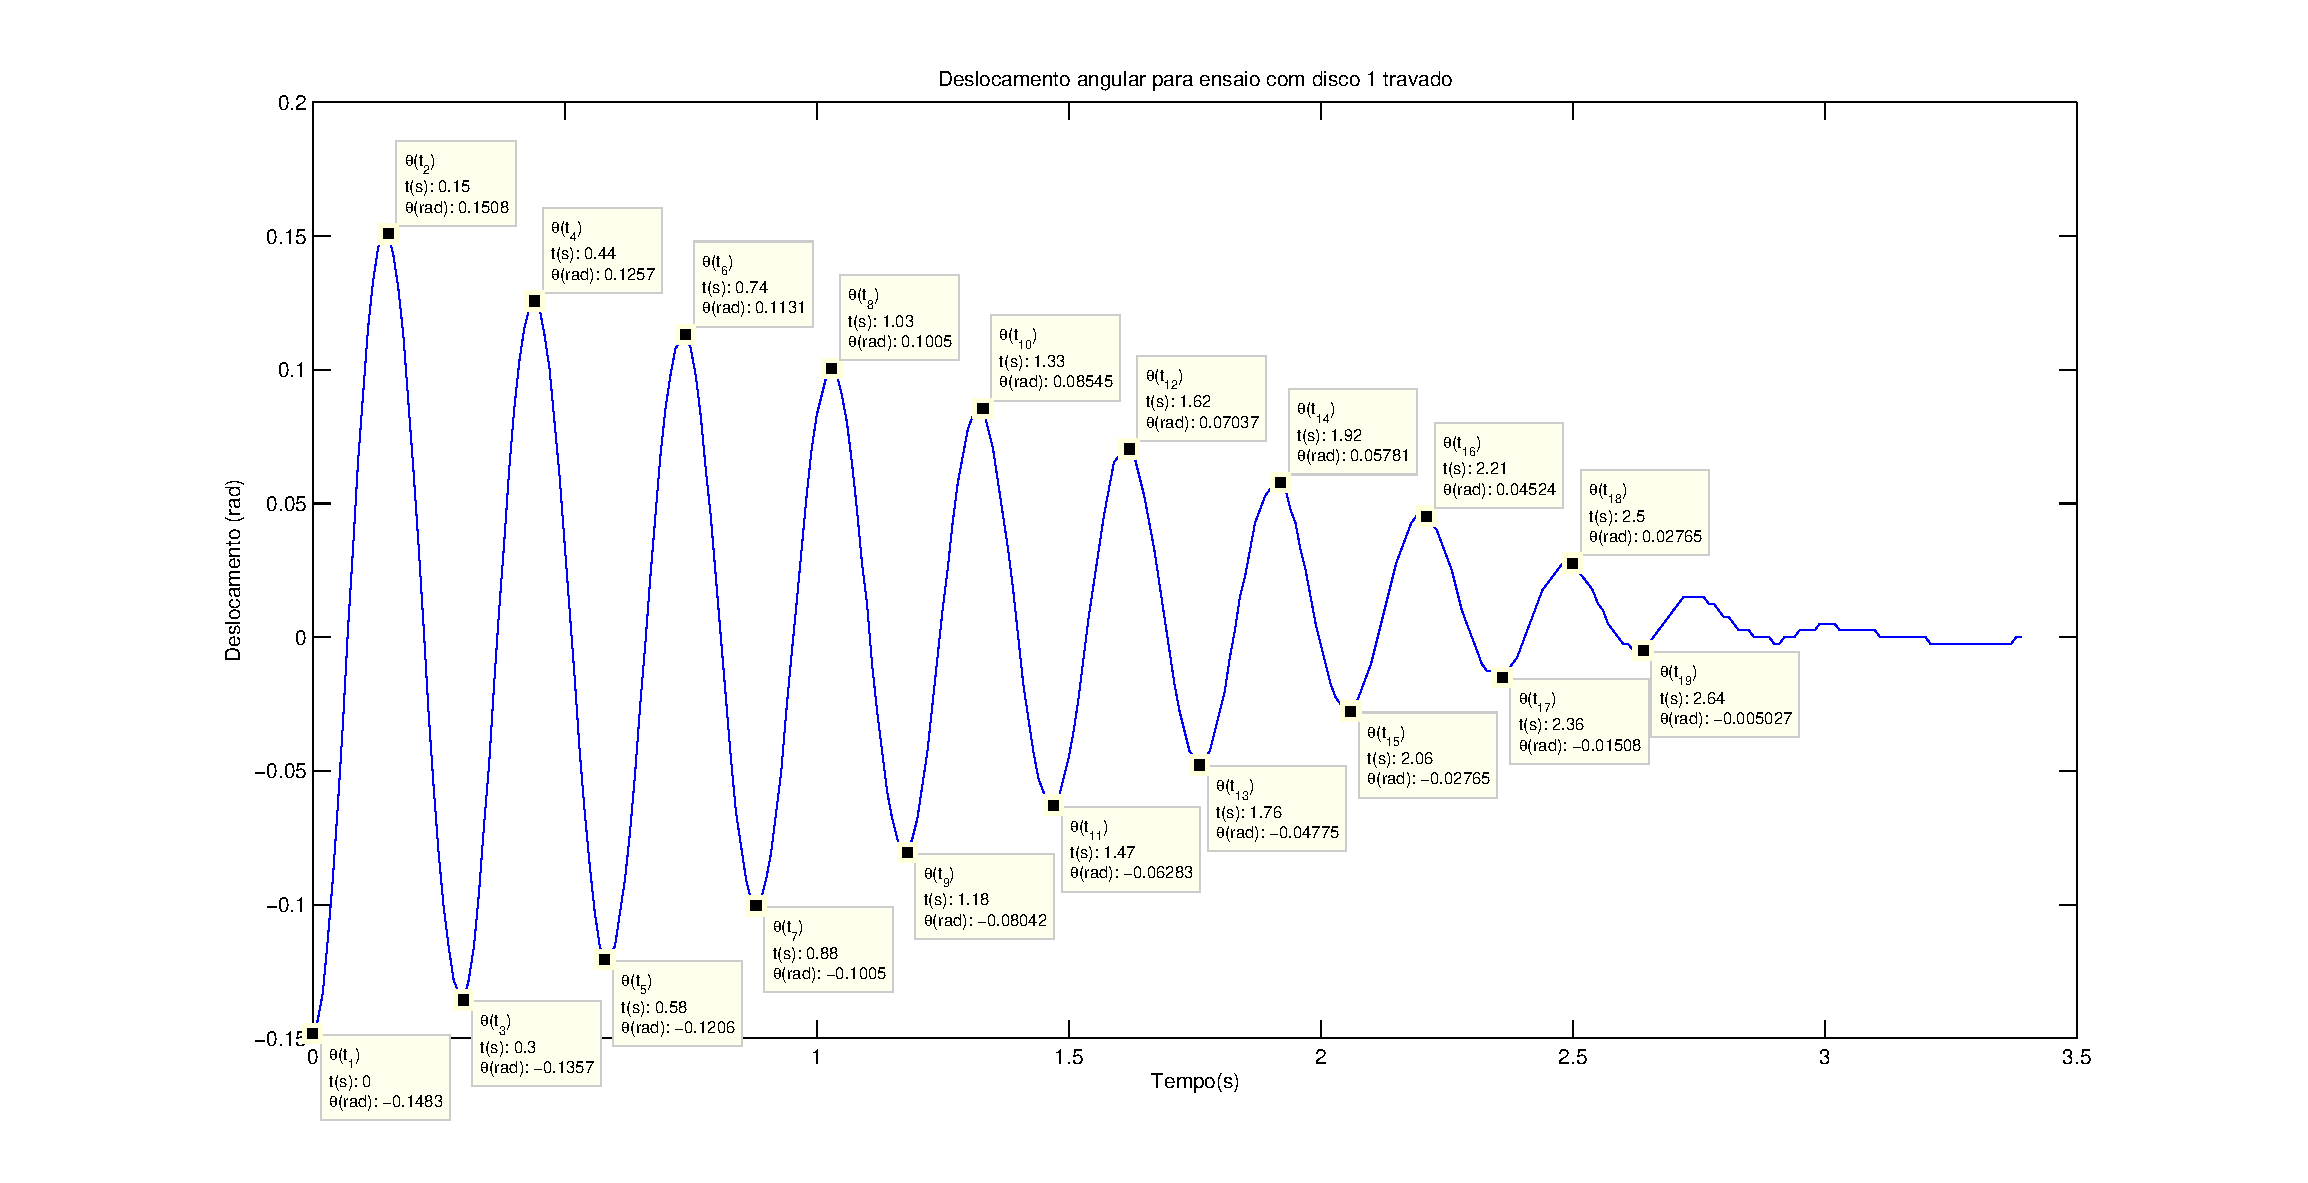
\includegraphics[width=0.8\linewidth]{../disco1travado}
	\caption{Pontos de relevância para deslocamento angular em oscilação do disco 2 (lado sem motor)}
	\label{fig:disco1travado}
\end{figure}

%TODO: Frequências naturais e fatores de amortecimento
A partir dos pontos obtidos pelas curvas de oscilação, conseguimos obter os parâmetros de frequência natural e fator de amortecimento para os discos 1 e 2, sendo dados por $\omega_{n1}=%TODO
$, $\xi_1=%TODO
$, $\omega_{n2}=%TODO
$ e $\xi_2=%TODO
$.

Conforme o roteiro\cite{bb:roteiro}, as frequências naturais e os fatores de amortecimento levam às equações \ref{eq:kappa1}, \ref{eq:kappa2}, \ref{eq:b1} e \ref{eq:b2}. 
\begin{equation}
\label{eq:kappa1}
\kappa=\omega_{n1}^2J_1
\end{equation}
\begin{equation}
\label{eq:kappa2}
\kappa=\omega_{n2}^2J_2
\end{equation}
\begin{equation}
\label{eq:b1}
b_1=2\xi_1\omega_{n1}J_1-\frac{K^2}{R}
\end{equation}
\begin{equation}
\label{eq:b2}
b_2=2\xi_2\omega_{n2}J_2
\end{equation}

A partir da equação \ref{eq:b1b2} e a soma das equações \ref{eq:b1} e \ref{eq:b2}, encontramos o valor uma combinação de $J_1$ e $J_2$, que substituídos na soma ponderada das equações \ref{eq:kappa1} e \ref{eq:kappa2} leva ao valor $\kappa=%TODO
$. Por fim, encontramos os valores $J_1=%TODO
$ e $J_2=%TODO
$ substituindo o valor de $kappa$ nas equações \ref{eq:kappa1} e \ref{eq:kappa2}.

\section{Resultados finais}
A tabela \ref{tab:par} apresenta os valores obtidos para todas os parâmetros do sistema.
\begin{table}[H]
	\centering
	\caption{Parâmetros elétricos e mecânicos do sistema}
	\label{tab:valores}
	\begin{tabular}{|c|l|c|}
		\hline Símbolo & Significado & Valor \\ 
		\hline $J_1$ & Momento de inércia do disco 1 & $4.1188\cdot10^{-4}$\\ 
		\hline $J_2$ & Momento de inércia do disco 2 & $3.7095\cdot10^{-4}$\\
		\hline $b_1$ & Coeficiente de amortecimento do disco 1 & $4.2052\cdot10^{-5}$\\
		\hline $b_2$ & Coeficiente de amortecimento do disco 2 & $9.5110\cdot10^{-4}$\\ 	 
		\hline $\kappa$ & Constante elástica da mola & $0.1708$\\ 
		\hline $V$ & Tensão no motor & $12$\\ 
		\hline $K$ & Constante mecânica do motor & $0.0663$\\ 
		\hline $R$ & Resistência do motor somada à resistência inserida para medida & $4.0709$ \\
		\hline $L$ & Indutância do motor & $0$ \\ 	
		\hline 
	\end{tabular} 
\end{table}

Com todos os parâmetros necessários calculados, substituindo os valores em \ref{eq:ss}, obtemos a planta dada pela equação na forma de estados \ref{eq:ssval}.

\begin{equation}
\label{eq:ssval}
\left[ \begin{array}{c}
\dot{x_1} \\
\dot{x_2} \\
\dot{x_3} \end{array} \right]
=
\left[ \begin{array}{ccc}
0 & 1 & -1 \\
-414.7063 & -2.7235 & 0 \\
-460.4577 & 0 & -2.5639 \end{array} \right]
\left[ \begin{array}{c}
x_1 \\
x_2 \\
x_3  \end{array} \right]
+
\left[ \begin{array}{c}
0 				\\
39.5397 	\\
0				\end{array} \right]
V
\end{equation}

\begin{thebibliography}{widestlabel}
	\bibitem{bb:roteiro}{Roteiro do experimento disponibilizado para os alunos}
\end{thebibliography}
\end{document}

